\documentclass[12pt, A4]{article}
\usepackage[utf8]{inputenc}
\usepackage{graphicx}
\usepackage{geometry}
\usepackage{hyperref}
\usepackage{datetime}
\bibliographystyle{unsrt}
\usepackage{float}


\title{PH456 Complex Systems Essay: Belousov–Zhabotinsky Reactions}
\author{Anton Gashi: 201914462 \\ Email: \href{anton.gashi.2019@uni.strath.ac.uk}{anton.gashi.2019@uni.strath.ac.uk} \\ Github: \href{https://github.com/AntonGashi/Computation_Class}{/Essay Code, Results, Animations \& Latex/}}
\date{\today}

\begin{document}
\begin{titlepage}
\clearpage\maketitle
\thispagestyle{empty}
\end{titlepage}

\abstract

Belousov-Zhabotinsky reactions are a family of auto-catalytic and thus oscillatory chemical 
reactions that produce visible bifurcations. These reactions are chaotic and produce a strange 
attractor, meaning that slight variations in initial conditions result in exponentially larger difference 
in phase space separation over time. This chaotic system was researched, simulated and compared to 
relevant literature to better understand how this system works. The organator model was chosen to 
simulate this chemical reaction with phase space diagrams, limit cycle diagrams and animations 
produced to show the bifurcations and chaos.

\section{Introduction} % (fold)
\label{sec:Introduction}

The Belousov-Zhabotinsky (BZ) reaction is an example of a oscillatory chemical 
reaction that exhibits self organised spirals on a 2D plane. 
This reaction usually entails an organic substrate and a catalyst-indicator, 
and through the mathematical model of the oregonator (and other models) a wide variety of chemicals 
can be used to create this experiment \cite{chen2000mathematical}.
This experiment is usually carried out by adding energy into the system, either 
stirring or a flow of the chemicals entering the experiment, this can also 
be simulated computationally with random noise and starting conditions to keep it in the 
chaotic regime \cite{petrov1993controlling}.
The behaviour of the BZ reaction, which is chaotic, can be described by 
the strange attractor in phase space and by an infinite number of 
unstable periodic oscillations if plotted against time. This means that the 
BZ reaction is extremely sensitive to initial conditions and also that the structure of 
the attractor are generally self similar. In an oregonator simulation, \cite{mukesh1993modelling}, 
the fractal dimension of the BZ reaction was calculated to be between 5.2 and 5.8, with 
the largest Lyapunov exponent being around $\lambda = 0.55$. This further suggests that 
the BZ reaction is a strange attractor and chaotic.


\section{Theory} % (fold)
\label{sec:Theory}

The BZ experiment is a class of experiments, but is usually given in the form of: 
\begin{equation}
  3CH_2(CO_2H)(aq)+4BrO^-_3(aq)\rightarrow 4Br^-(aq)+9CO_2(g)+6H_2O(I)
\end{equation}

The reaction is a pair of auto-catalytic process's in which Bromine is an intermediary in the 
scheme, the Bromine will increase if there is enough reactants in the chemical solution and 
will produce bromide ions. Although this increases another reactant which depletes the Bromine, 
and after the Bromine is depleted the other reactant is depleted also leading it full circle \cite{lister1995classic}.
The experiment also shows temporal and spatial changes in colour, clearly showing 
the oscillations and bifurcations. In experiments, i.e. not a simulation, the BZ reaction 
goes though three stages in the lifespan of the experiment; transitional period, 
induction period and main period. When a stage switches from the transitional period to 
the induction period there is a bifurcation from a monostable state to a bistable state. 
In relation to figures \ref{fig:frame0}, \ref{fig:frame300} and \ref{fig:frame300_12}, the bifurcation 
is the colour change in the 'chemicals' \cite{chen2000mathematical}.


\begin{figure}[H]
  \begin{center}
    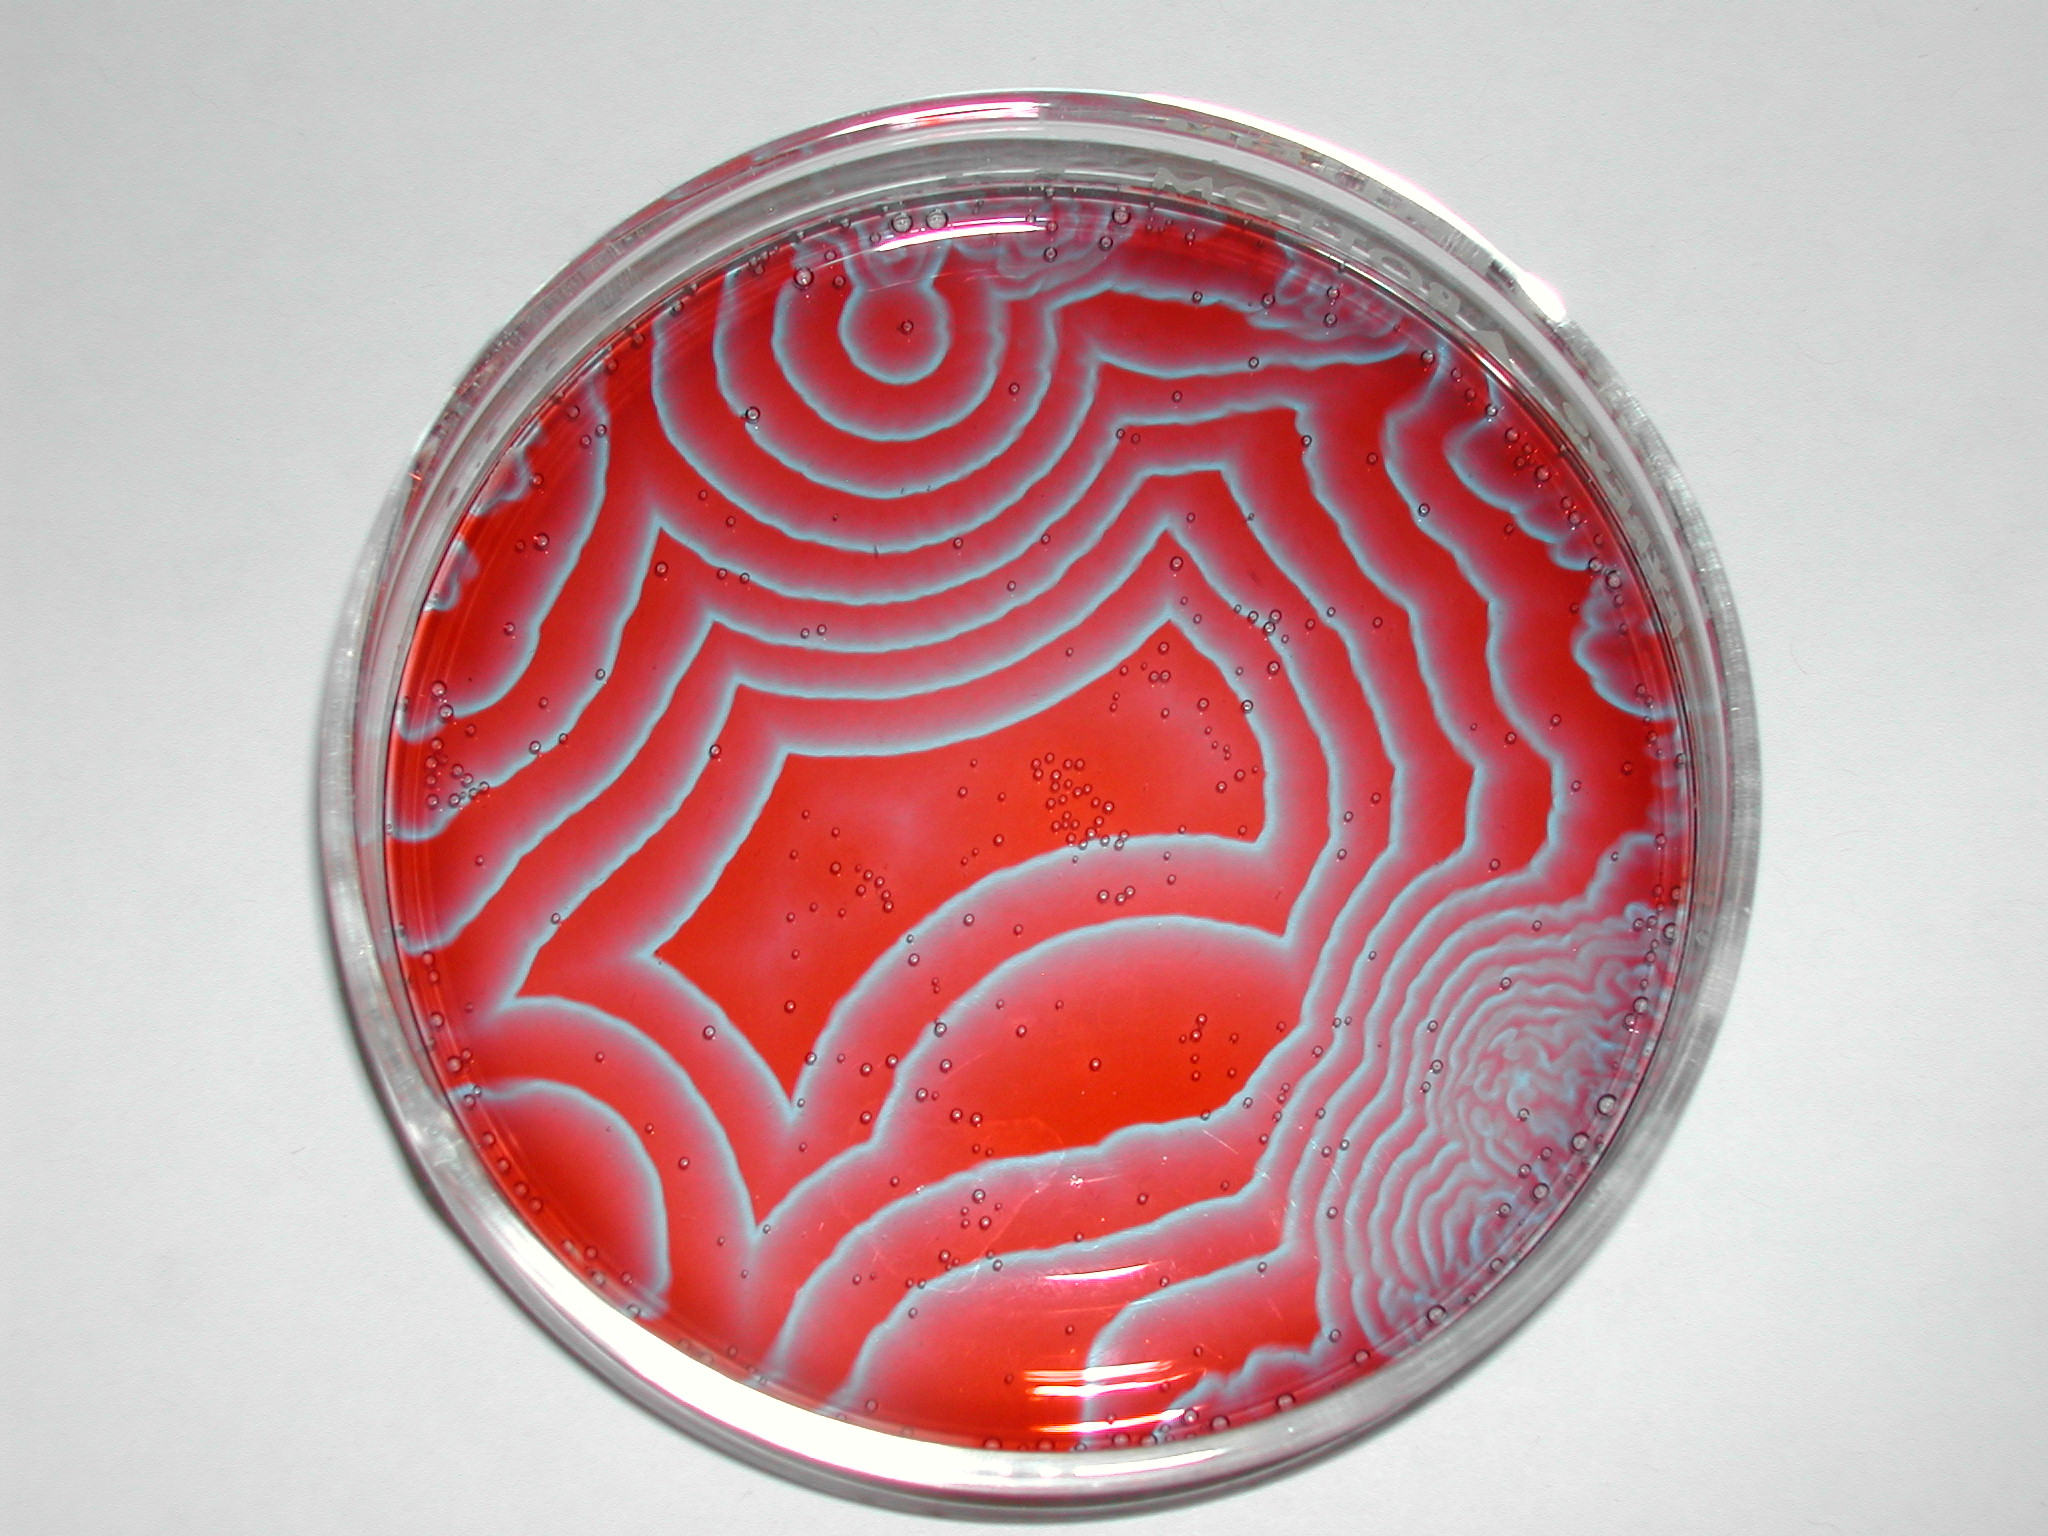
\includegraphics[width=0.5\textwidth]{bz.jpg}
  \end{center}
  \caption{Image of a physical Belousov-Zhabotinsky reaction in a Petri dish.}
  \label{fig:}
\end{figure}



\subsection{Computational Model} % (fold)
\label{sub:Computational Model}

% subsection subsection name (end)

The method being used to simulate the BZ reaction was presented by Ball(1994)\cite{ball1996designing}, 
and it's described as a series of chemical equations \cite{turner2009simple}:

\begin{equation}\label{eq1}
  A+B \rightarrow 2A
\end{equation}
\begin{equation}\label{eq2}
  B+C \rightarrow 2B
\end{equation}
\begin{equation}\label{eq3}
  C+A \rightarrow 2C
\end{equation}


This reaction is self referential as for an amount of A to exist there needs to be an 
amount of B, for B to exist there needs to be an amount of C, and finally for C to exist there 
needs to be an amount of A. These can be used to generate time dependant equations as such:

\begin{equation}\label{eq4}
  a_{t+1}=a_t+a_t(b_t-c_t)
\end{equation}
\begin{equation}\label{eq5}
  b_{t+1}=b_t+b_t(c_t-a_t)
\end{equation}
\begin{equation}\label{eq6}
  c_{t+1}=c_t+c_t(a_t-b_t)
\end{equation}

Note that $a_t$ is being used to denote the absolute amount of A at a specific time $t$, and 
similarly for $b_t$ and $c_t$. Also $a_{t+1}$ denotes the absolute amount of A at a specific time 
plus 1 time step.


For this Essay's visualisation of the BZ reaction a discretised grid (usually 300x300) was used to mimic 
the reaction that would usually take place on a Petri dish. Since the space is discretised 
the act of diffusion was averaged by a convolved 9x9 grid, that is to say the absolute 
amount of 'chemical' at any point on the grid was summed on the 9x9 grid and divided evenly 
at each point. Adjusting equations \ref{eq4},\ref{eq5},\ref{eq6} the terms $\alpha,\beta,\gamma$ 
can be added to give control over the absolute amount of each 'chemical' at each time step:

\begin{equation}\label{eq7}
  a_{t+1}=a_t+a_t(\alpha b_t-\gamma c_t)
\end{equation}
\begin{equation}\label{eq8}
  b_{t+1}=b_t+b_t(\beta c_t-\alpha a_t)
\end{equation}
\begin{equation}\label{eq9}
  c_{t+1}=c_t+c_t(\gamma a_t-\beta b_t)
\end{equation}

\section{Results}
\label{sec:Results}

\begin{figure}[b]
  \begin{center}
    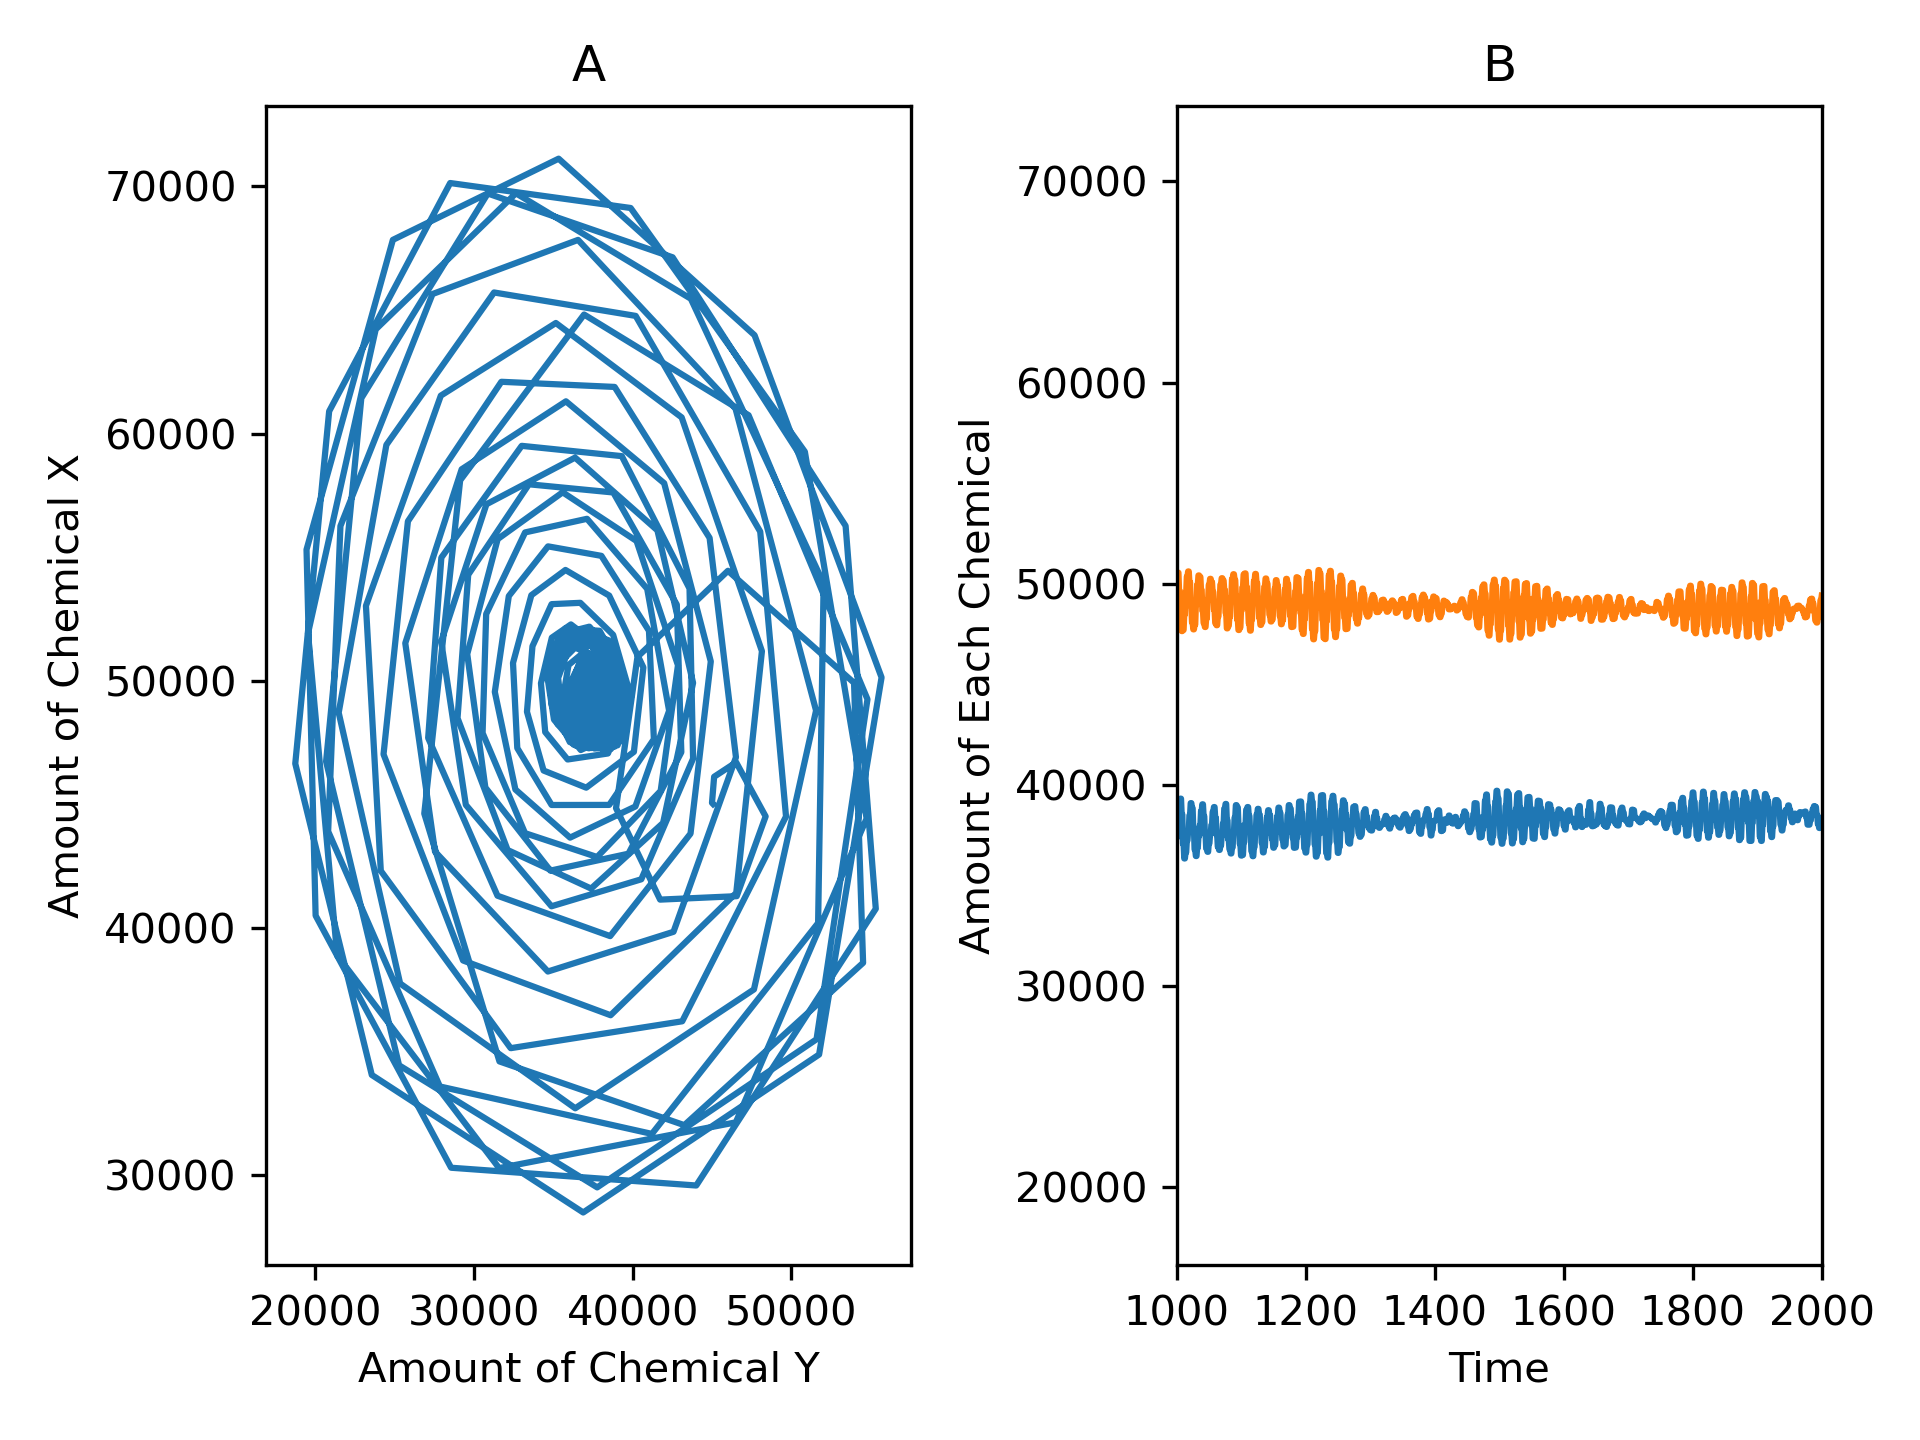
\includegraphics[width=0.6\textwidth]{first_pic.png}
  \end{center}
  \caption{A) Plot showing the attractor nature of the system. B) Plot showing the unstable periodic oscillations over time. With $\alpha,\beta,\gamma =1$.}
  \label{fig:first}
\end{figure}

\begin{figure}[b]
  \begin{center}
    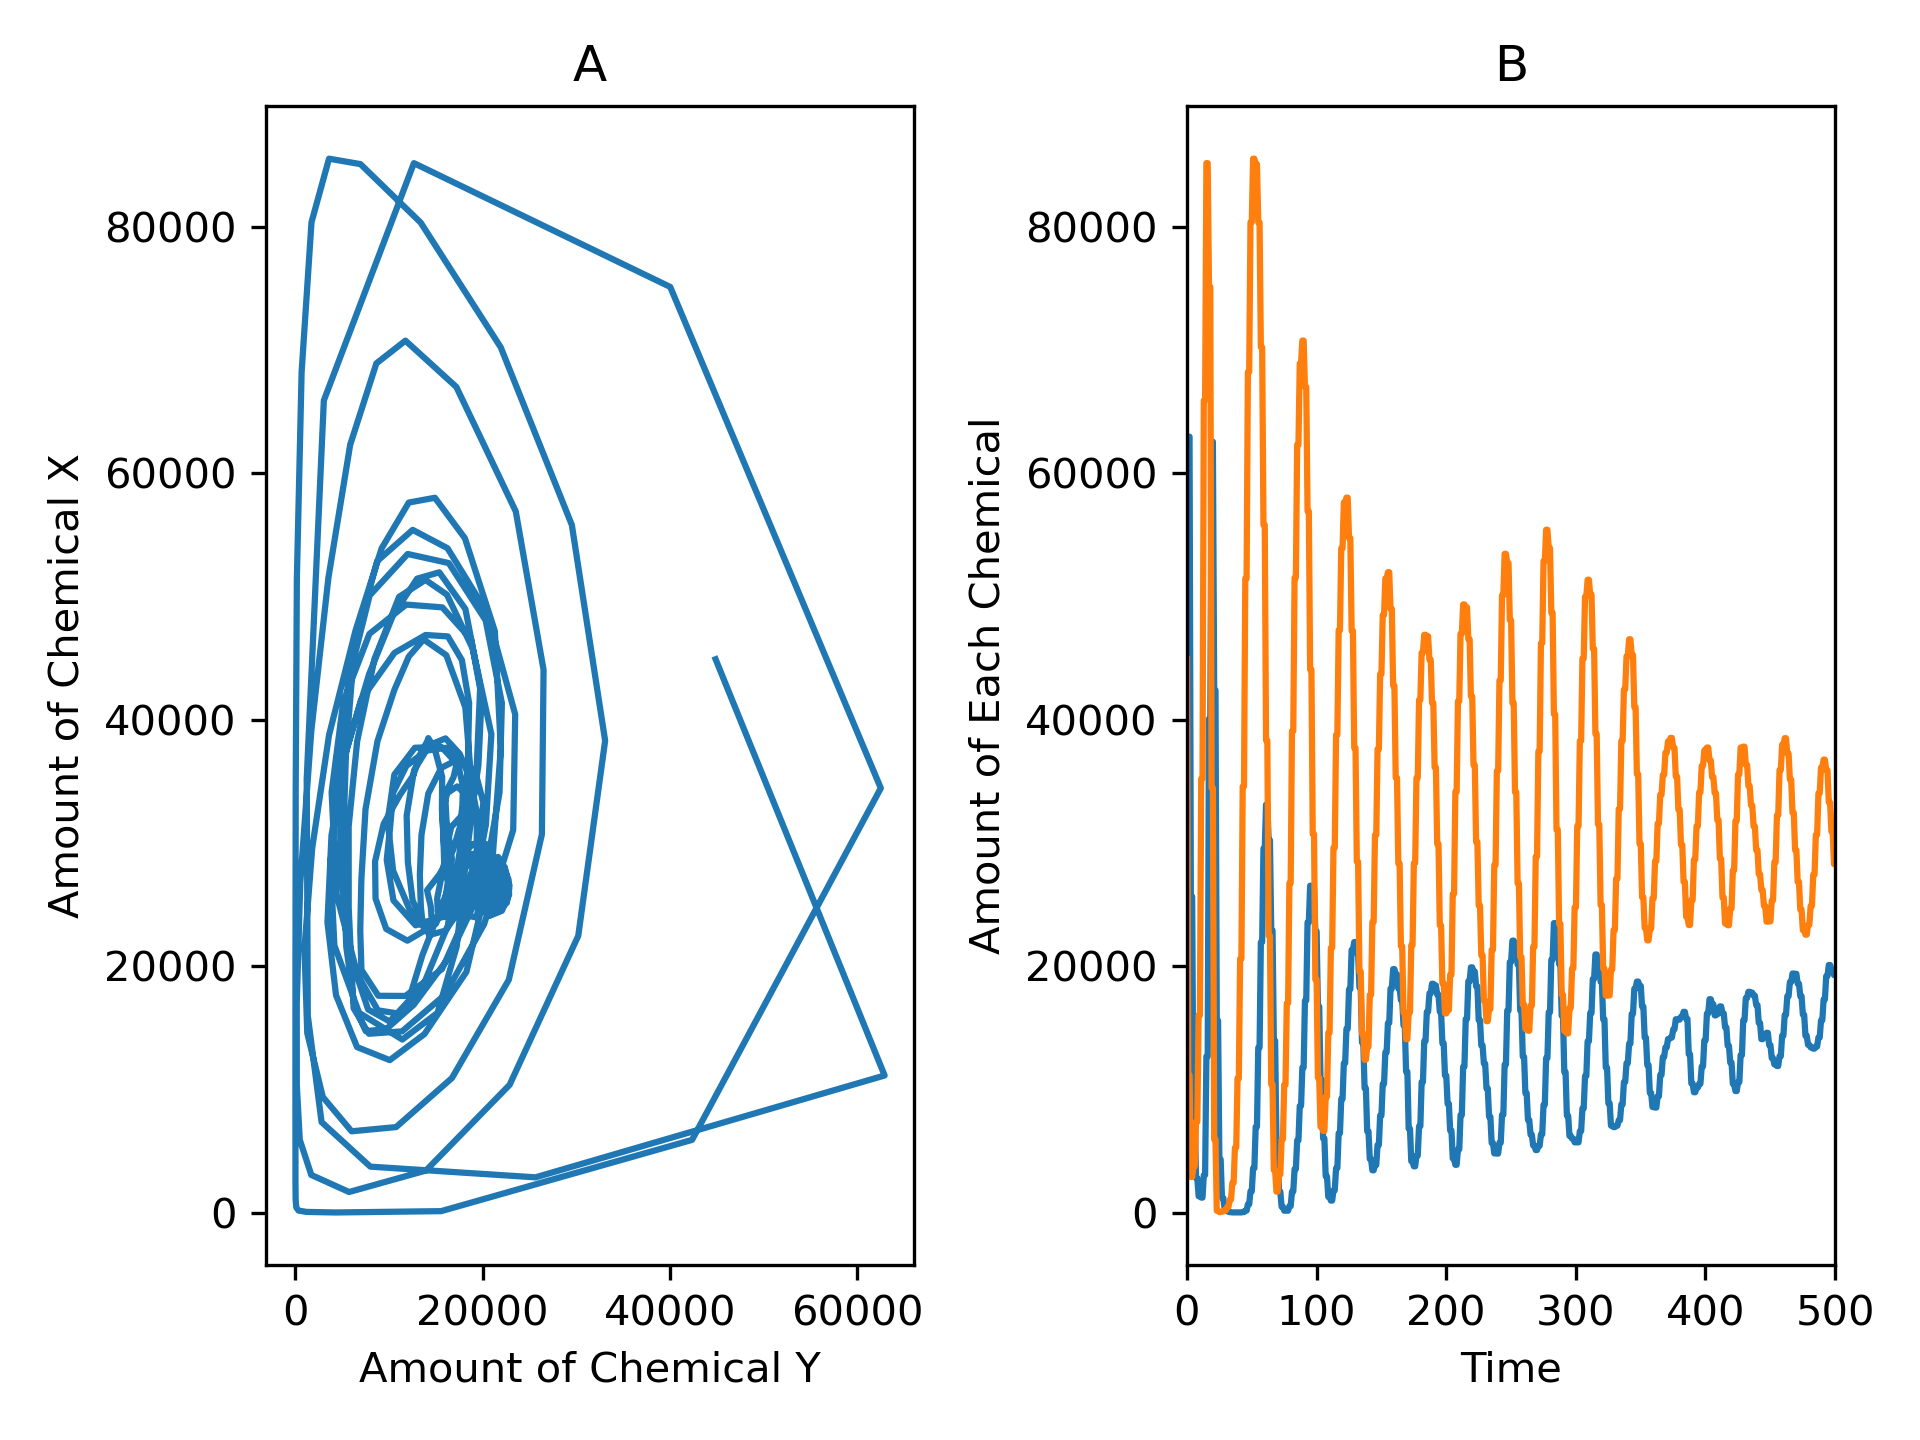
\includegraphics[width=0.6\textwidth]{organator.png}
  \end{center}
  \caption{A) Plot showing the attractor nature of the system resembling the Brusselator in a stable regime. B) Plot showing the unstable periodic oscillations over time .With $\alpha=1.7, \beta,\gamma =1$.}
  \label{fig:organatro}
\end{figure}

\begin{figure}[b]
  \begin{center}
    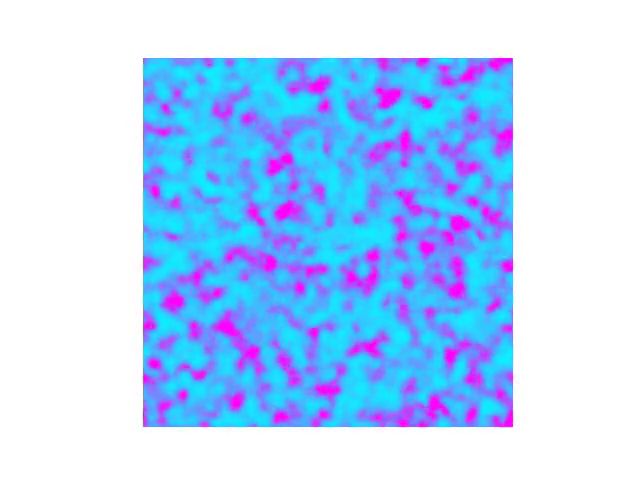
\includegraphics[width=0.6\textwidth]{frame_0.png}
  \end{center}
  \caption{Image of reaction at time step 0 with $\alpha,\beta,\gamma =1$, can be seen with no pattern yet apart from initial random noise entered into the system.}
  \label{fig:frame0}
\end{figure}

\begin{figure}[b]
  \begin{center}
    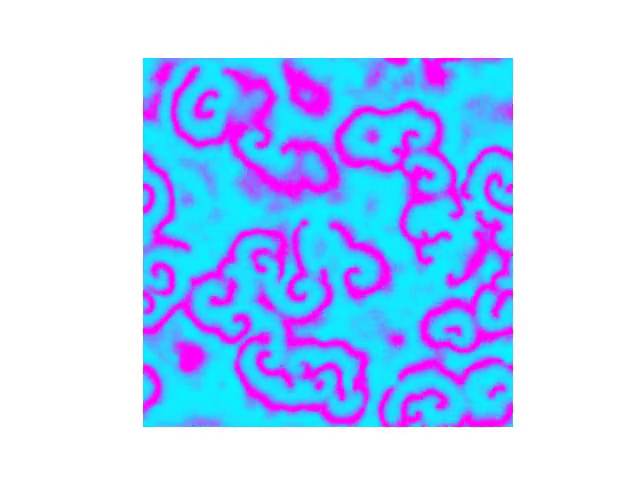
\includegraphics[width=0.6\textwidth]{frame_300.png}
  \end{center}
  \caption{Image of reaction at time step $\approx$ 300 with $\alpha,\beta,\gamma =1$, can be seen exhibiting wave fronts characteristic of the BZ reaction.}
  \label{fig:frame300}
\end{figure}

\begin{figure}[b]
  \begin{center}
    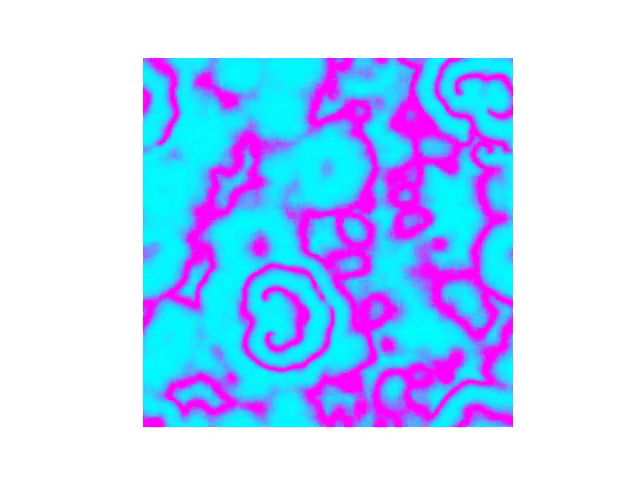
\includegraphics[width=0.6\textwidth]{frame_300_12.png}
  \end{center}
  \caption{Image of reaction at time step $\approx$ 300 with $\alpha=1.2 ,\beta,\gamma =1$}
  \label{fig:frame300_12}
\end{figure}

\begin{figure}[b]
  \begin{center}
    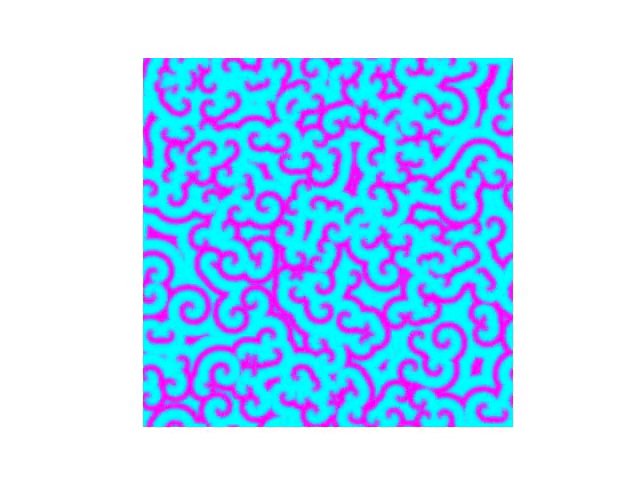
\includegraphics[width=0.6\textwidth]{frame_300_311.png}
  \end{center}
  \caption{Image of reaction at time step $\approx$ 300 with $\alpha=3 ,\beta,\gamma =1$}
  \label{fig:frame_300_311}
\end{figure}


\begin{figure}[b]
  \begin{center}
    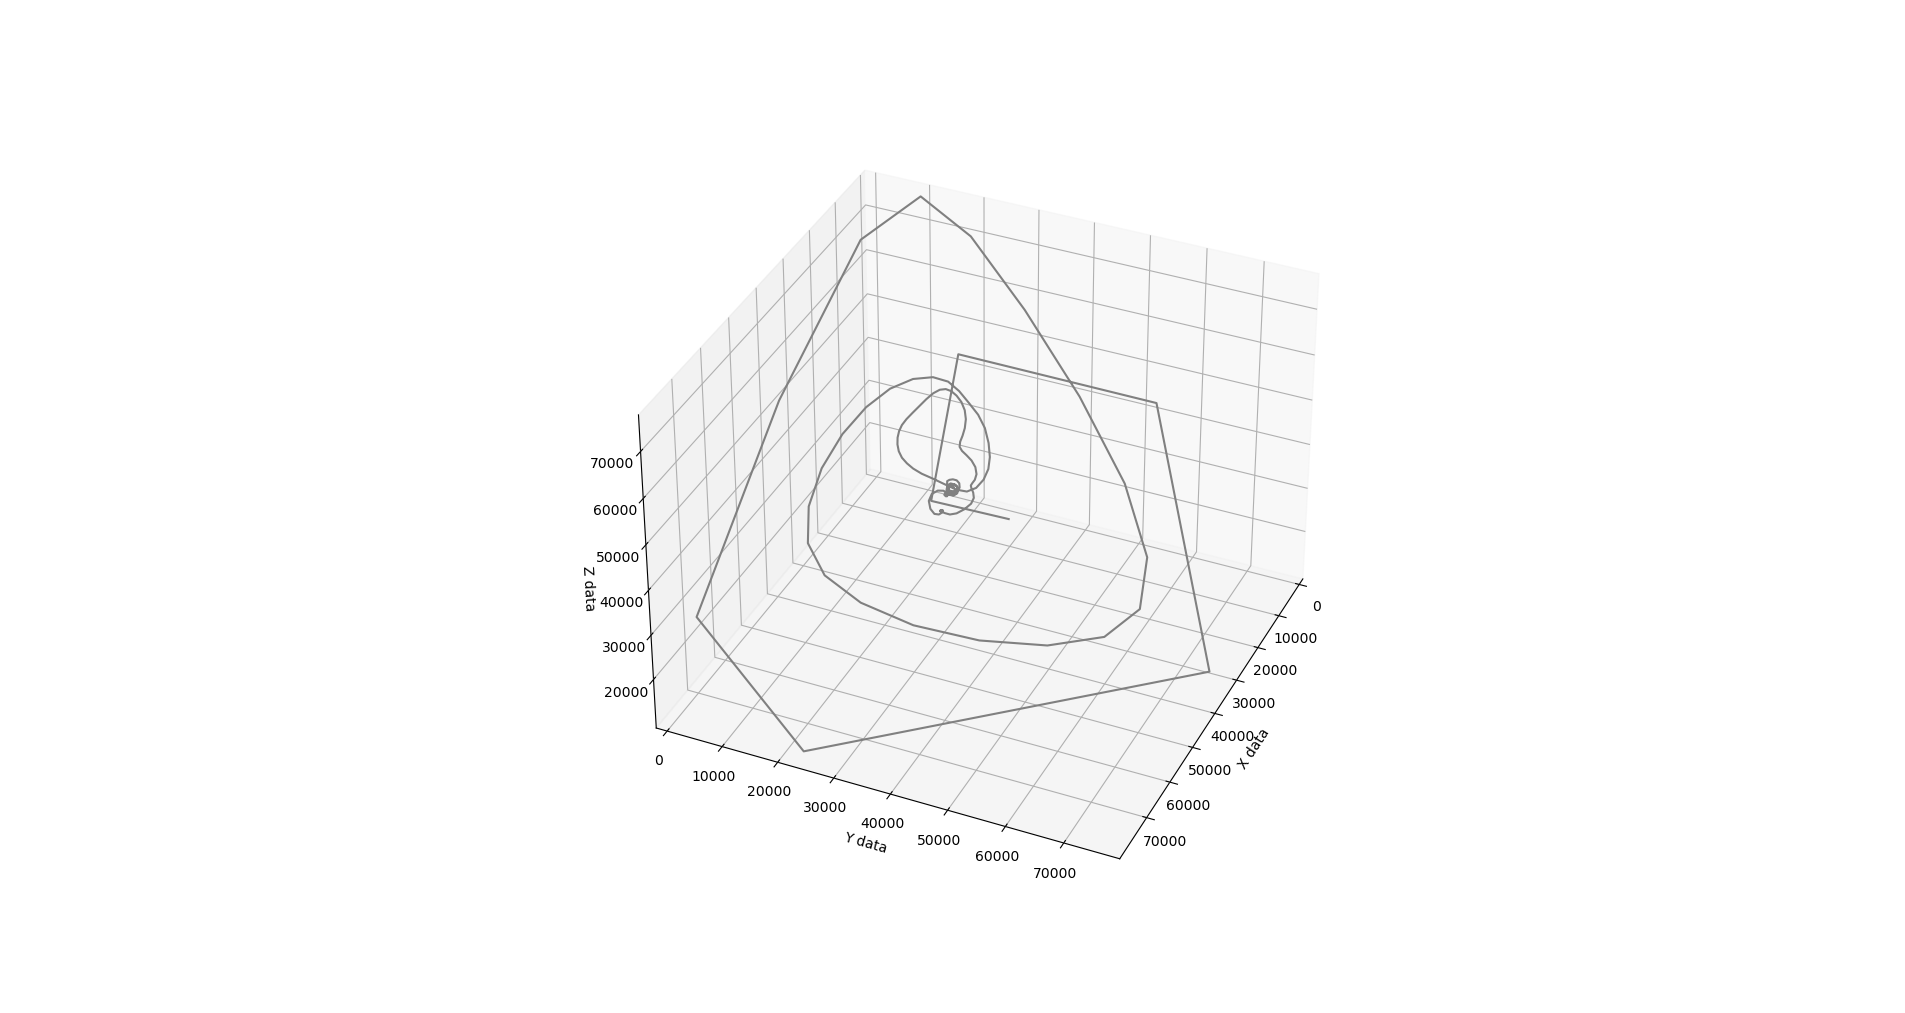
\includegraphics[width=1.2\textwidth]{3d.png}
  \end{center}
  \caption{3D plots of absolute amount of $a_t, b_t, c_t$ with $\alpha,\beta,\gamma =1$}
  \label{fig:3d}
\end{figure}

\begin{figure}[b]
  \begin{center}
    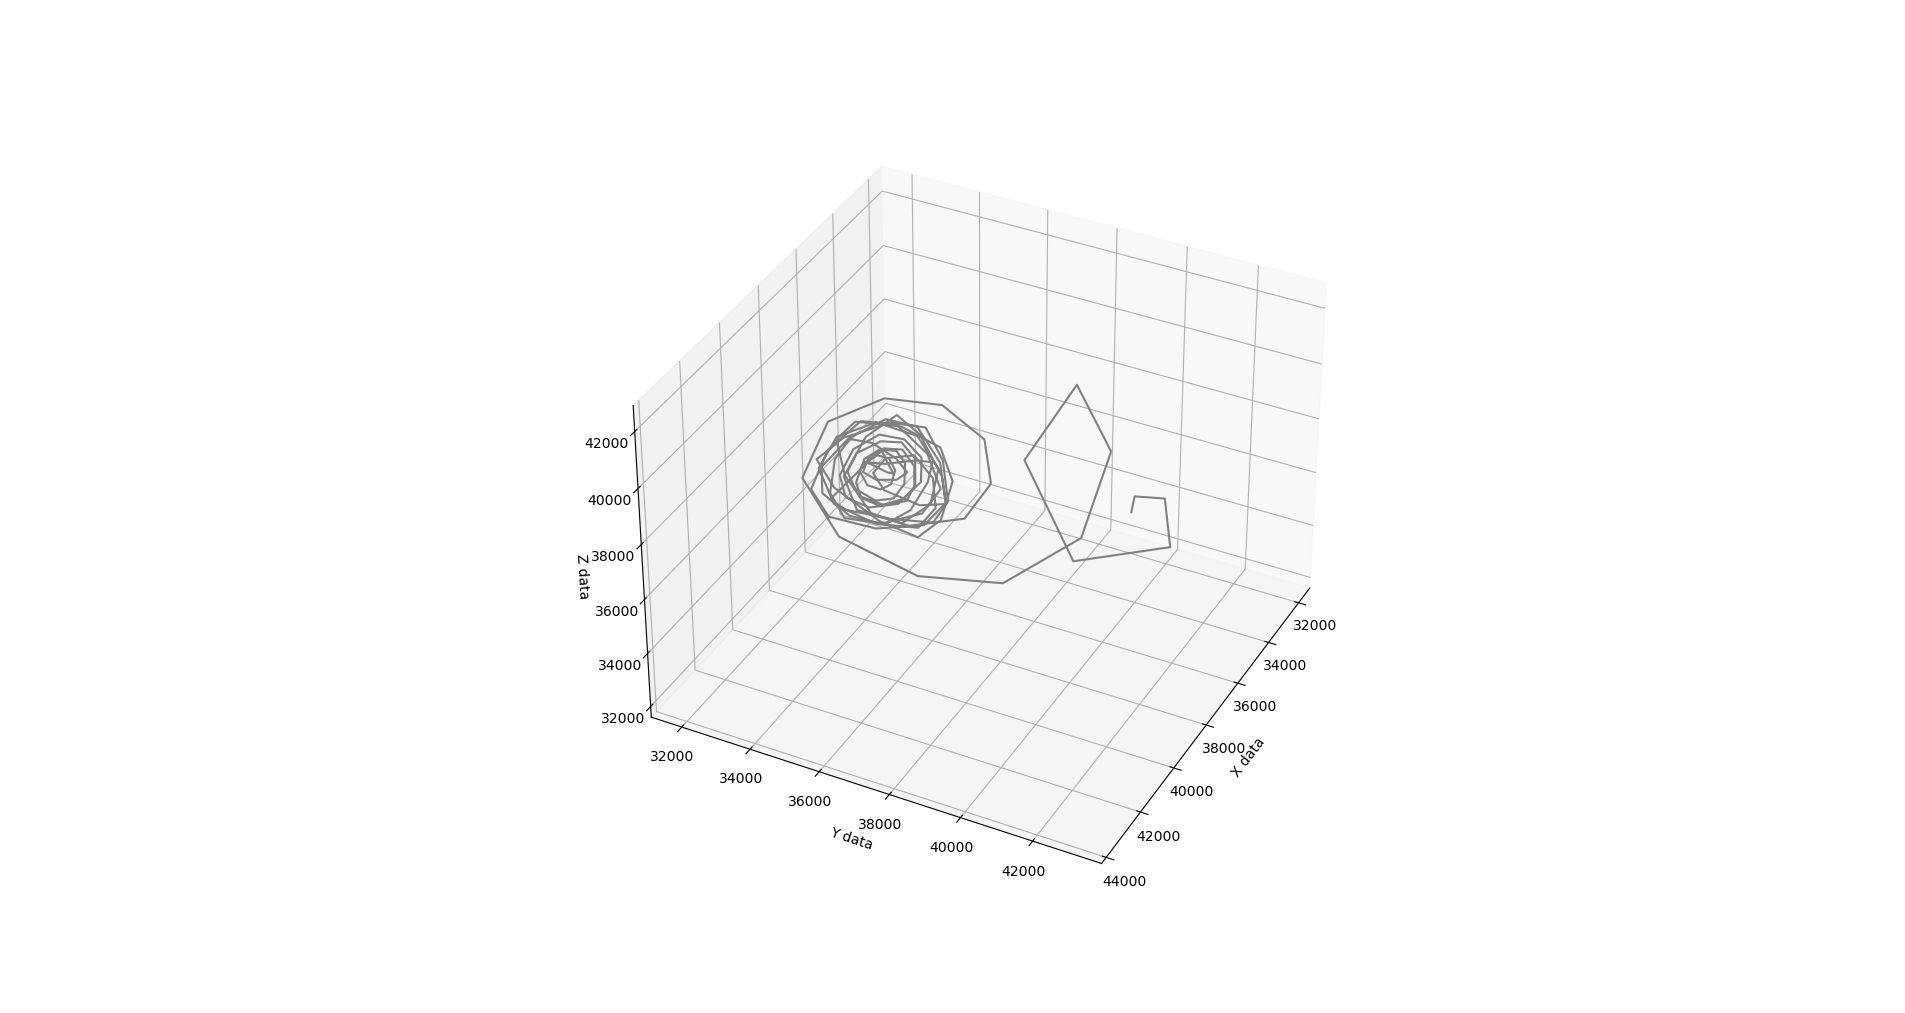
\includegraphics[width=1.2\textwidth]{3d2.png}
  \end{center}
  \caption{3D plots of absolute amount of $a_t, b_t, c_t$ with $\alpha=1.2 ,\beta,\gamma =1$}
  \label{fig:3d2}
\end{figure}

\begin{figure}
  \begin{center}
    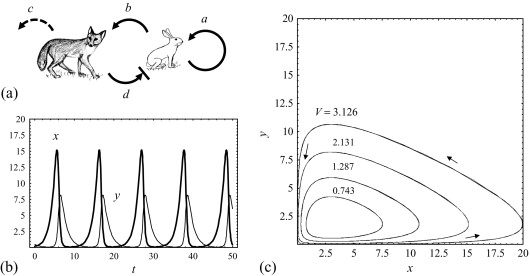
\includegraphics[width=0.95\textwidth]{pred_pray.jpg}
  \end{center}
  \caption{Lotka–Volterra system taken from Pattern formations and oscillatory phenomena\cite{kinoshita2013pattern}}
  \label{fig:pred_pray}
\end{figure}


The general trend that can be seen in figures \ref{fig:frame300},\ref{fig:frame300_12} and \ref{fig:frame_300_311}
and can be seen in further detail if the animations are seen, shows that after a period of time 
the absolute amounts of each 'chemical' and therefor colour seem to stabilise into repeating waves. 
This is somewhat intuitive as chaotic attractors are locally unstable but globally stable 
once the graph has 'fallen' into the attractor, this behaviour can be seen in figures 
\ref{fig:first}A and \ref{fig:organatro}A. Another behaviour that can be observed from figures 
\ref{fig:first}B and \ref{fig:organatro}B is a recurrent non periodic behaviour as discussed in the notes.

As described in section \ref{sec:Theory} the amount of each chemical is dependant on relative 
amounts of the other chemicals in the experiment, this is analogous to the predator prey model.
The predator prey model is governed by the Lotka-Volterra equations which denote the change in 
predator prey populations as such\cite{kinoshita2013pattern}:

\begin{equation}
  \dot{x}=x(a-by)
  \label{eq:LV1}
\end{equation}

\begin{equation}
  \dot{y}=-y(c-dx)
  \label{eq:LV2}
\end{equation}

In figure \ref{fig:pred_pray} it can be seen that for certain starting values of the particular 
predator prey model, for a period of time, follows the same pattern as figure \ref{fig:organatro}.
This growth and death of a population can particularly be seen in figure \ref{fig:pred_pray}(b) and 
figure \ref{fig:organatro}(B)(from $0\rightarrow 300$ time steps)

\section{Conclusion} % (fold)
\label{sec:Conclusion}

In conclusion the Belousov-Zhabotinsky reaction is an example of a system that's in a thermodynamic 
non-equilibrium, this produces nonlinear chemical oscillations. Due to this these reactions 
evolve chaotically under the condition of being perturbed slightly, whilst also 
being an attractor making this experiment a strange attractor. Also as mentioned in the notes 
if the sign of the Lyapunov exponent is positive, then the system is believed to be chaotic.

One draw back of using the computational method that was used is that the time steps 
are fixed, this produced plots that are more quantised rather than being continuous. 
The advantage is that it's simple to implement and runs relatively quickly, plus it 
uses pre made packages like scipy.signal.convolve2d which can easily deal with wrapping, so in 
effect the simulations showing the reactions are taking place on a torus.


\bibliography{references}
\end{document}
